\subsection{Chassi}
Vid design av chassit användes CAD-programmet SolidWorks 2012 för att göra
3D-modeller över chassits olika delar. En prototyp modellerades i SolidWorks och
tillverkades för att användas till olika tester innan det slutliga chassit
skulle designas och tillverkas.

\subsubsection{Material}
Chassit är gjort av ett lätt skivmaterial som består av två tunna “pappskivor”
med skumplast emellan. Skivorna är 3,1 mm tjocka och är lätta att klippa, skära
och limma. Projektgruppen har fått skivorna från Björn-Åke Sköld, som driver
företaget Sköld Design, för att göra en prototyp av svävaren. Materialet
användes till prototypen men även till den slutliga svävaren. Dysorna till
fläktarna är gjorda av papprör och träramen som håller ihop höljet som döljer
elektroniken är av furu. Till kjolen användes ett ripstop-tyg som är ett
slitstarkt tunt tyg som används bl.a. till drakar.

\subsubsection{Prototyp}
Arbetet inleddes med att göra en CAD-modell över prototypen. Den gjordes dubbelt
så stor jämfört med den svävare som en tidigare projektgrupp har byggt.
Björn-Åke trodde nämligen att man skulle kunna göra en lite större svävare men
som ändå är lättare än den gamla när man använder hans material. Prototypen blev
800x570 mm och 100 mm hög. Tanken var att den gamla svävaren skulle fästas
ovanpå prototypen för att se om den kunde lyfta och sväva då. En annan tanke var
att även kjolen skulle ha testats på prototypen för att sedan kunna flyttas över
till den slutliga svävaren. Eftersom det inte skulle bli helt lätt att fästa den
gamla svävaren på prototypen testades prototypen direkt med de lyftfläktar som
skulle användas. Den kunde då lyfta och hållas svävande trots att ingen kjol
användes. Kjolen designades som en variant av fingerkjol bestående av flera
segment men hann inte sys innan en idé på en ny design dök upp.

\subsubsection{Ny design}
Efter ett möte med Björn-Åke då han fick se prototypen och CAD-modellen av
kjolen bestämdes att både chassit och kjolen skulle konstrueras om. Detta för
att kjolsegmenten blev för små att sy och att kjolen i sin helhet inte skulle
kunna hålla kvar luften så att ett lufttryck kunde erhållas. I den nya designen
kunde höjden halveras på svävaren och bredden ökas 3 cm så att den blev
stabilare. Det nya chassit har en bagkjol istället eftersom det är lättare att
sy en sådan kjol och den kan dessutom hålla kvar luften på ett bättre sätt så
ett lufttryck erhålls. En bagkjol är inte lika flexibel som en fingerkjol när
det gäller att ta sig över hinder men i detta projekt är bagkjolen tillräckligt
flexibel.

Kjolen sitter fast i en plattform med kardborreband och eftersom det försvinner
mycket luft vid kardborrefästena har inte några hål gjorts i kjolen. På så vis
erhålls även ett lufttryck i kjolen som gör att svävaren kan bära en större
totalvikt. Plattformen som kjolen är fäst runt är 800x600 mm och består av två
plattor av det lätta skivmaterialet. Den undre plattan är lite mindre än den
övre och de sitter ihop med distanser för att få en luftspalt på 10 mm mellan
plattorna. Träramen är till för att fästa fläktar, motorer och elektronik i. Den
sitter fast i plattformen med kardborreband och håller även ihop höljet som
döljer elektroniken med kardborreband. Svävaren är uppbyggd på ett modulärt sätt
och de olika delarna är placerade på ett sätt som ger låg tyngdpunkt. Den är
även uppbyggd symmetriskt med en jämn viktfördelning över hela svävarens
bottenyta. En 3D-modell över svävaren visas i Figur \ref{fig:CAD_Hover}.
 
\begin{figure}[htbp!] 
\centering 
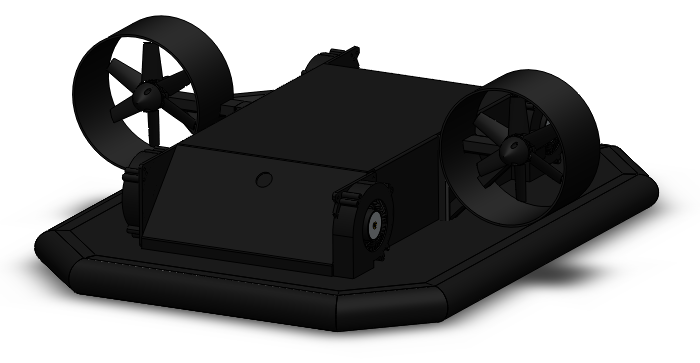
\includegraphics[width=8cm]{../includes/figures/CAD_Hovercraft.png} 
\caption{3D-modell över svävaren} 
\label{fig:CAD_Hover} 
\end{figure}

\subsubsection{Vidareutveckling}
I en vidareutveckling av svävaren skulle materialet kunna bytas ut mot ett mer
hållbart och vattentåligt material. Skivmaterialet har en tendens att slitas
sönder när delarna ska tas isär vid kardborrefästena. Träramen som är av furu
skulle kunna bytas ut till ett lättare träslag som balsaträ. Genom att skala upp
modellen kan en större svävare göras med samma design. Men det som behöver
tänkas på då är att de fläktar och motorer som väljs klarar av den nya vikten.
